%%%%%%%%%%%%%%%%%%%%%%%%%%%%%%%%%%%%%%%%%
% Beamer Presentation
% LaTeX Template
% Version 1.0 (10/11/12)
%
% This template has been downloaded from:
% http://www.LaTeXTemplates.com
%
% License:
% CC BY-NC-SA 3.0 (http://creativecommons.org/licenses/by-nc-sa/3.0/)
%
%%%%%%%%%%%%%%%%%%%%%%%%%%%%%%%%%%%%%%%%%

%----------------------------------------------------------------------------------------
%	PACKAGES AND THEMES
%----------------------------------------------------------------------------------------

\documentclass{beamer}

%----------------------------------------------------------------------------------------
%   PACKAGES

\usepackage{hyperref}
\usepackage{multimedia}
\usepackage{graphicx}
\usepackage{makecell}
%----------------------------------------------------------------------------------------



\mode<presentation> {

% The Beamer class comes with a number of default slide themes
% which change the colors and layouts of slides. Below this is a list
% of all the themes, uncomment each in turn to see what they look like.

%\usetheme{default}
%\usetheme{AnnArbor}
%\usetheme{Antibes}
%\usetheme{Bergen}
%\usetheme{Berkeley}
\usetheme{Berlin} %<-
%\usetheme{Boadilla} %<-
%\usetheme{CambridgeUS}
%\usetheme{Copenhagen}
%\usetheme{Darmstadt}
%\usetheme{Dresden}
%\usetheme{Frankfurt}
%\usetheme{Goettingen}
%\usetheme{Hannover}
%\usetheme{Ilmenau} %<-
%\usetheme{JuanLesPins}
%\usetheme{Luebeck}
%\usetheme{Madrid} %<-
%\usetheme{Malmoe}
%\usetheme{Marburg}
%\usetheme{Montpellier}
%\usetheme{PaloAlto}
%\usetheme{Pittsburgh}
%\usetheme{Rochester}
%\usetheme{Singapore}
%\usetheme{Szeged}
%\usetheme{Warsaw}

% As well as themes, the Beamer class has a number of color themes
% for any slide theme. Uncomment each of these in turn to see how it
% changes the colors of your current slide theme.

%\usecolortheme{albatross}
%\usecolortheme{beaver}
%\usecolortheme{beetle}
%\usecolortheme{crane}
%\usecolortheme{dolphin}
%\usecolortheme{dove}
%\usecolortheme{fly}
%\usecolortheme{lily}
\usecolortheme{orchid} %<-
%\usecolortheme{rose}
%\usecolortheme{seagull}
%\usecolortheme{seahorse}
%\usecolortheme{whale}
%\usecolortheme{wolverine}

%\setbeamertemplate{footline} % To remove the footer line in all slides uncomment this line
%\setbeamertemplate{footline}[page number] % To replace the footer line in all slides with a simple slide count uncomment this line

\setbeamertemplate{navigation symbols}{} % To remove the navigation symbols from the bottom of all slides uncomment this line
}

\addtobeamertemplate{navigation symbols}{}{%
	\usebeamerfont{footline}%
	\usebeamercolor[fg]{footline}%
	\hspace{1em}%
	\insertframenumber/\inserttotalframenumber
}

\usepackage{graphicx} % Allows including images
\usepackage{booktabs} % Allows the use of \toprule, \midrule and \bottomrule in tables

%----------------------------------------------------------------------------------------
%	TITLE PAGE
%----------------------------------------------------------------------------------------

\title[A Comparison of Synthetic-to-Real Domain Adaptation Techniques]{A Comparison of Synthetic-to-Real Domain Adaptation Techniques} % The short title appears at the bottom of every slide, the full title is only on the title page

\author{Peter Trost} % Your name
\institute[Universität Tübingen] % Your institution as it will appear on the bottom of every slide, may be shorthand to save space
{
Eberhard Karls Universität Tübingen \\
Mathematisch-Naturwissenschaftliche Fakultät\\
Wilhelm-Schickard-Institut für Informatik\\
Lernbasierte Computer Vision\\ % Your institution for the title page
\medskip
\textit{peter.trost@student.uni-tuebingen.de} % Your email address
}
\date{\today} % Date, can be changed to a custom date

\AtBeginSubsection[]{
	\begin{frame}
		\frametitle{Overview}
			\tableofcontents[currentsubsection]
	\end{frame}
}

\begin{document}

\begin{frame}
\titlepage % Print the title page as the first slide
\end{frame}

\begin{frame}
\frametitle{Overview} % Table of contents slide, comment this block out to remove it
\tableofcontents % Throughout your presentation, if you choose to use \section{} and \subsection{} commands, these will automatically be printed on this slide as an overview of your presentation
\end{frame}

%----------------------------------------------------------------------------------------
%	PRESENTATION SLIDES
%----------------------------------------------------------------------------------------
\begin{frame}
	\frametitle{Overview}
	thesis goals:
	\begin{enumerate}
		\item adapt images from synthetic to real domain using three different techniques
		\item compare adaptation performance of these techniques
	\end{enumerate}
\end{frame}

%------------------------------------------------
\section{Introduction}
%------------------------------------------------

\subsection{Motivation}

\begin{frame}
	\frametitle{Autonomous driving}
	\begin{itemize}
		\item use Deep Neural Networks
		\item need lots of data to perform well
		\item supervised learning yields best models
		\item labeling may be inaccurate (human annotators)
		\item data acquisition expensive
	\end{itemize}
\end{frame}

\subsection{Foundations}

\begin{frame}
%todo show code for mapping of pixel values to train ids
\frametitle{Domain Adaptation}
\begin{columns}[c]
	\column{.5\textwidth}
	\begin{figure}
		\centering
		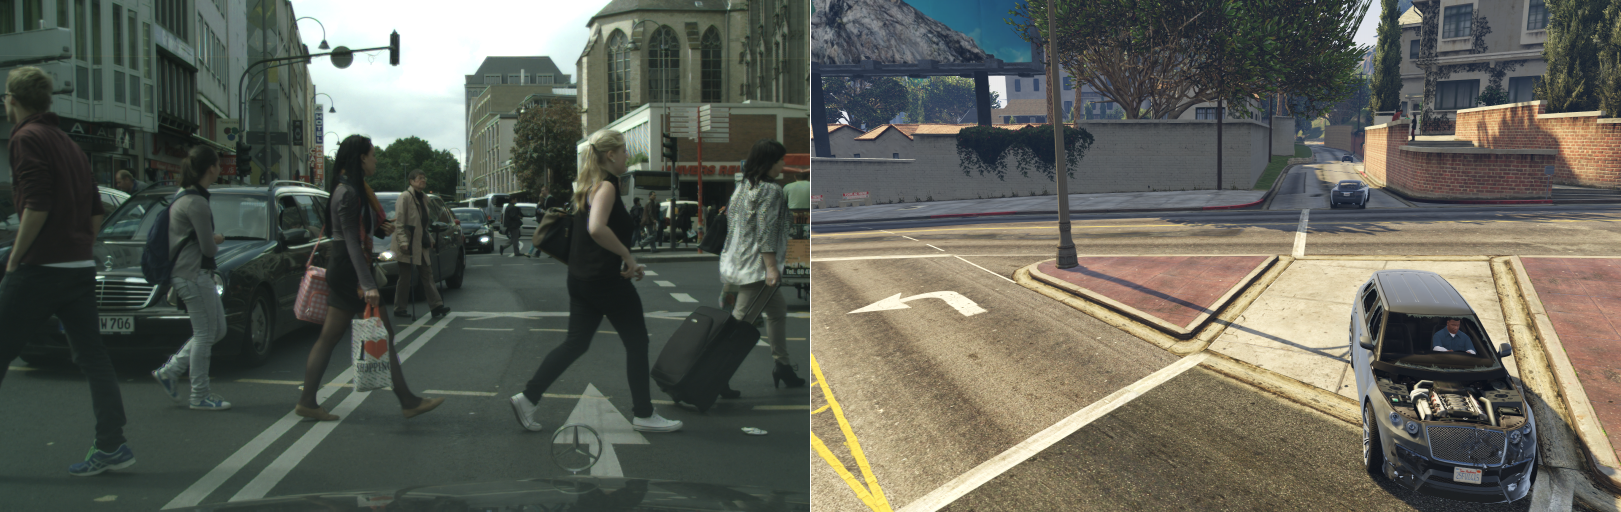
\includegraphics[width=1.1\textwidth]{../images/DA_examples_cityscapes_gta.png}
		\caption{example images of the two domains relevant for this thesis. Real domain (left, Cityscapes dataset) and synthetic domain (right, GTA5 dataset)}
		%todo cite cityscapes
		%todo cite GTA5
	\end{figure}
	\column{.5\textwidth}
	\begin{itemize}
		\item may have a lot of data in one domain but not as much in another related one
		\item train machine learning model on the first domain
		\item perform domain adaptation: transfer that model to the other domain
	\end{itemize}
\end{columns}
\end{frame}

%todo add video if possible
%\begin{frame}
%	\frametitle{Autonomous driving}
%	\movie[poster]{}{tesla_smartsummon_fail.avi}
%\end{frame}

\begin{frame}
	\frametitle{Generative Adversarial Networks}
	\begin{itemize}
		\item discriminator learns data distribution from training data (real)
		\item generator generates images (fake)
		\item GANs implement two player game:\\
		generator tries to fool the discriminator into labeling generated images as real
	\end{itemize}
\end{frame}
%todo add more example images

\begin{frame}
\frametitle{Generative Adversarial Networks}
\begin{figure}
	\centering
	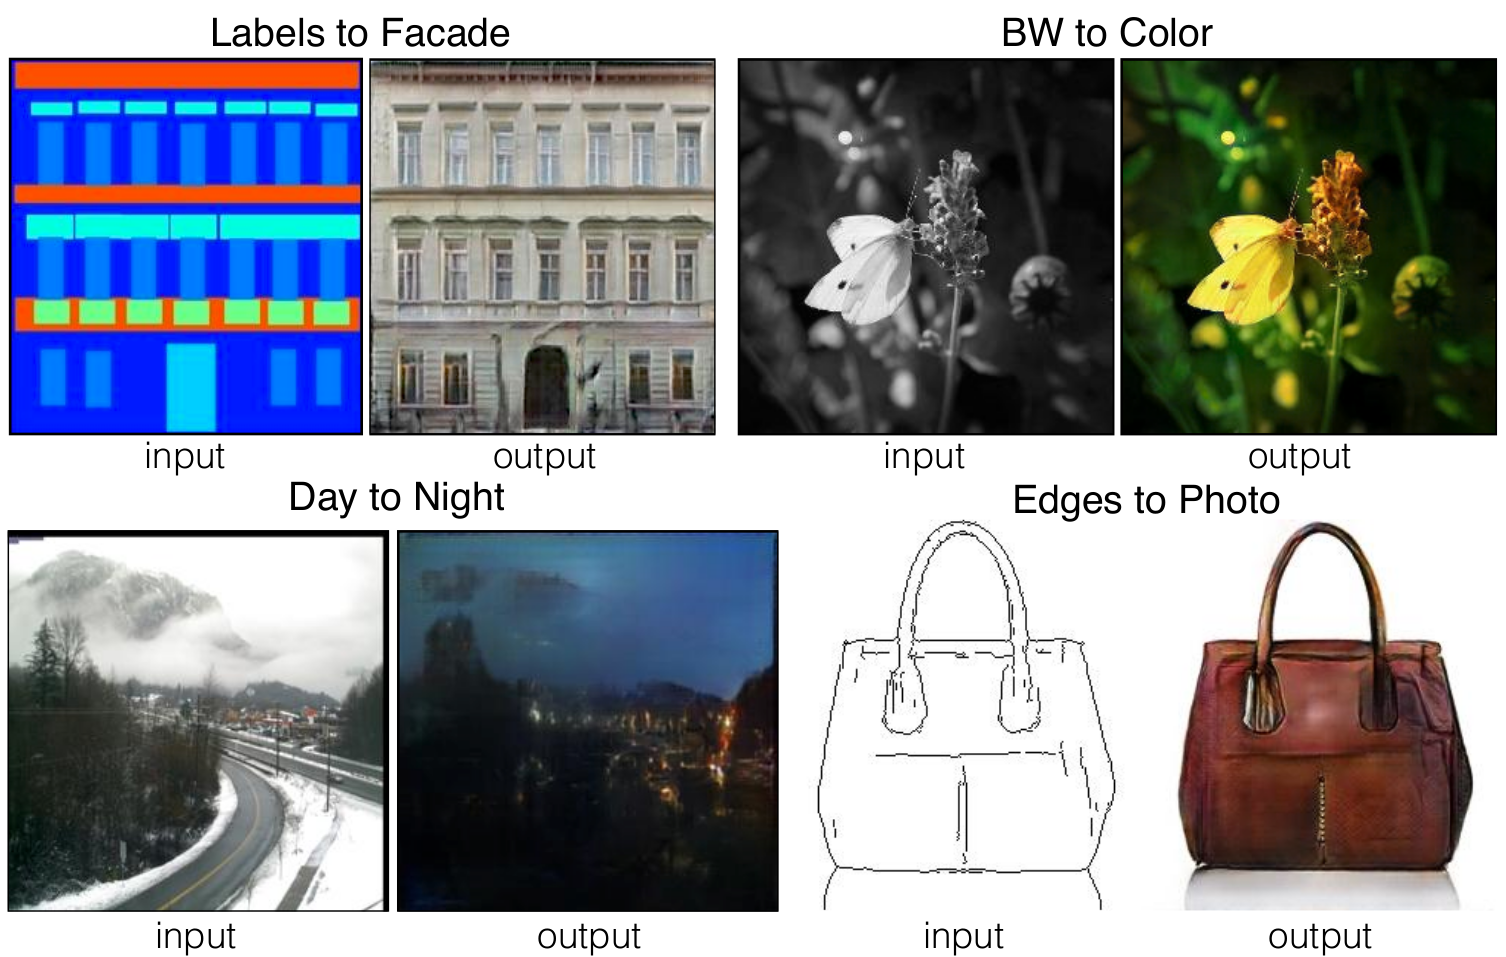
\includegraphics[width=0.7\textwidth]{../images/I2I_examples.png}
	\caption{Examples of conditional inputs and generated images (output) of conditional GANs as described in [add citation here]}
\end{figure}
%todo cite IZZE16 Image-to-Image translation
\end{frame}
%todo if need more time maybe include benefits and challenges of GANs

%------------------------------------------------
\section{Related Work}
%------------------------------------------------

\subsection{A Categorization}

\begin{frame}
\frametitle{Discrepancy based}
\begin{itemize}
	\item \textbf{class criterion:} uses class label information
	\item \textbf{statistic criterion:} align statistical distribution shift between source and target domains
	\item \textbf{architecture criterion:} modify the  network so it can learn more transferable features
	\item \textbf{geometric criterion:} bridges domains using their geometrical properties
\end{itemize}
\end{frame}

\begin{frame}
\frametitle{Adversarial based}
\begin{itemize}
	\item \textbf{generative models:} GANs
	\item \textbf{non-generative models:} feature extractor learns to distinguish between source and target domain, maps features to common space.
\end{itemize}
\end{frame}

\begin{frame}
\frametitle{Reconstruction based}
\begin{itemize}
	\item \textbf{encoder-decoder reconstruction:} combine encoder network for representation learning (features like edges, circle, etc.) and decoder network for data reconstruction
	\item \textbf{adversarial reconstruction:} use reconstruction error to make sure mapping from source to target and back to source results in the original datapoint
\end{itemize}
\end{frame}


%------------------------------------------------
\section{Domain Adaptation techniques}
%------------------------------------------------

\subsection{Motivation}
\begin{frame}
\frametitle{Why GANs?}
\begin{itemize}
	\item can generate images
	\item easier for humans to evaluate
	\item unsupervised learning
\end{itemize}
\end{frame}

\subsection{Techniques}

\begin{frame}
\frametitle{CycleGAN}
\begin{itemize}
	\item cycle-consistency loss: difference between source image and image translated to and then back from the target domain
	[add explanation graphic here]
	%todo add image of explanation graphic
\end{itemize}
\end{frame}

\begin{frame}
\frametitle{CyCADA}
\begin{itemize}
	\item additional semantic loss:
	\begin{enumerate}
		\item perform semantic segmentation on source image
		\item translate image to target domain
		\item perform semantic segmentation on that image
	\end{enumerate}
	difference between those two semantic maps describes the semantic loss
	[add visualization here]
	%todo add images for visualization
\end{itemize}
\end{frame}

\begin{frame}
\frametitle{SG-GAN}
\begin{itemize}
	\item additional gradient-sensitive objective: emphasize semantic boundaries by rendering distinct color/texture for each region
	[add visualization here]
	%todo add example image
\end{itemize}
\end{frame}

%------------------------------------------------
\section{Experiments}
%------------------------------------------------

\subsection{Methodology}

\begin{frame}
\frametitle{Comparison Benchmark: Semantic Segmentation}
\begin{itemize}
	\item task of segmenting an image into multiple sets of pixels (superpixels)
	\item goal: change representation of image in order to make it more meaningful or simpler to analyze
\end{itemize}
\end{frame}

\begin{frame}
\frametitle{Synthetic dataset: GTA5}
\begin{columns}[c]
\column{.5\textwidth}
	\begin{figure}
		\centering
		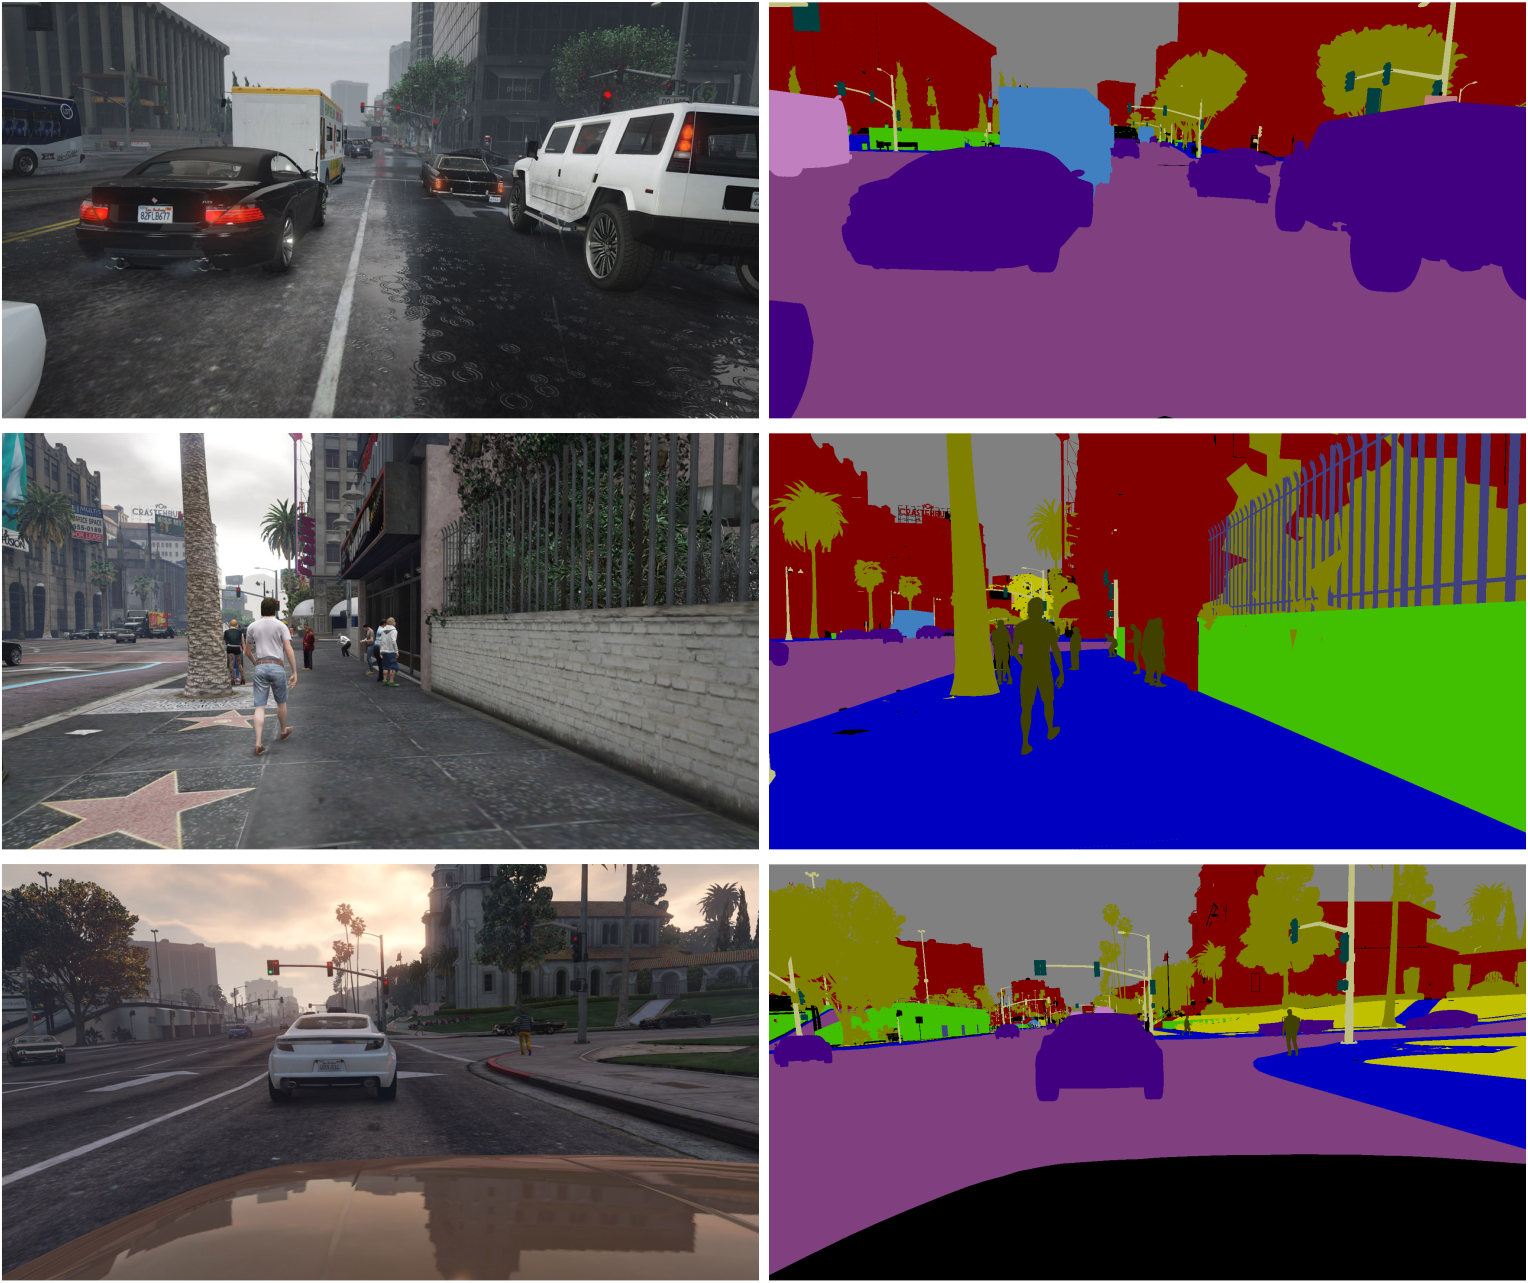
\includegraphics[width=\textwidth]{../images/p4d_example.png}
		\caption[GTA5 images]{GTA5 images (left) with corresponding annotations (right)}
	\end{figure}
\column{.5\textwidth}
	\begin{itemize}
		\item $\sim 25000$ images
		\item obtained from Grand Theft Auto V
	\end{itemize}
\end{columns}
\end{frame}
%todo citations
\begin{frame}
\frametitle{Real dataset: Cityscapes}
\begin{columns}[c]
	\column{.5\textwidth}
	\begin{figure}
		\centering
		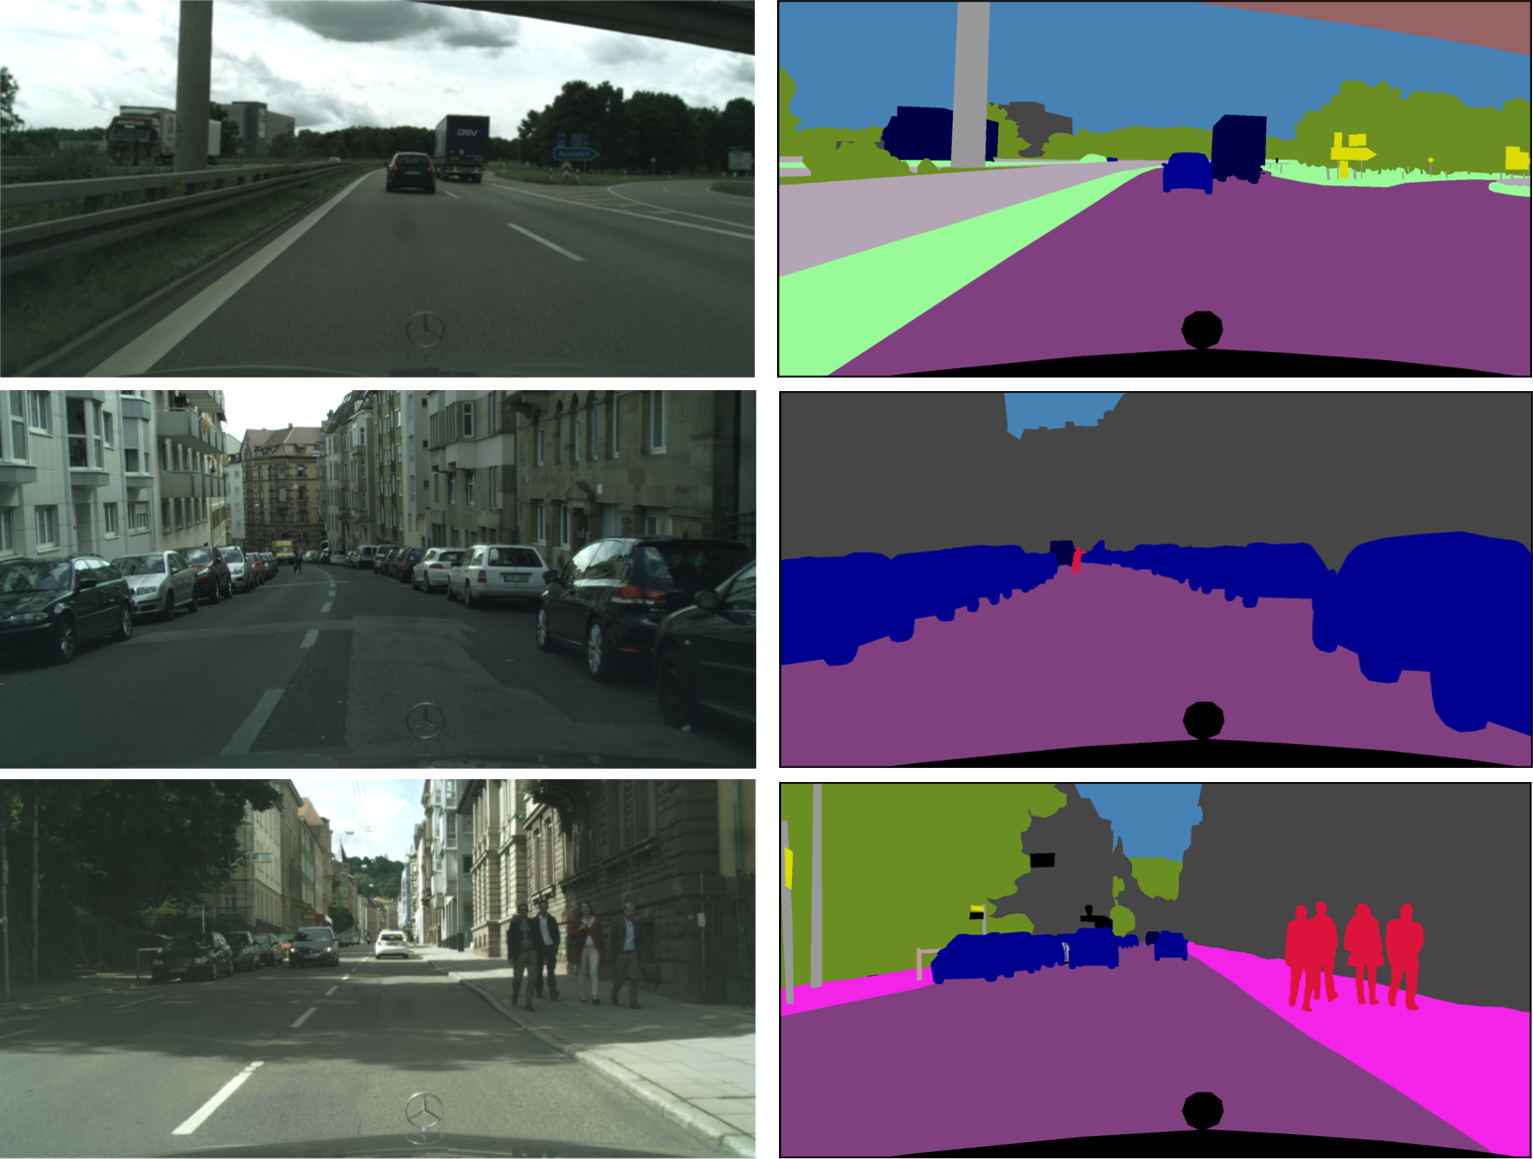
\includegraphics[width=\textwidth]{../images/cityscapes_example.png}
		\caption[Cityscapes images]{Cityscapes images (left) and corresponding fine annotations (right)}
	\end{figure}
	\column{.5\textwidth}
	\begin{itemize}
		\item $5000$ images with fine annotations
		\item $20000$ images with coarse annotations
	\end{itemize}
\end{columns}
\end{frame}

\begin{frame}
\frametitle{Image Translation}
\begin{itemize}
	\item sampleset of 500 images randomly chosen
	\item images translated using CycleGAN, CyCADA, SG-GAN
\end{itemize}
\end{frame}

\begin{frame}
\frametitle{Semantic Segmentation (DeepLabV3)}
\begin{itemize}
	\item DeepLabV3 performs semantic segmentation on translated images
	\item i.e. predicts label for every pixel in the image
\end{itemize}
\end{frame}

\begin{frame}
\frametitle{Evaluation}
\begin{itemize}
	\item using the Cityscapes provided code
	\item Intersection over Union
	\begin{align*}
		\frac{\text{predicted pixels} \cap \text{ground truth pixels}}{\text{predicted pixels} \cup \text{ground truth pixels}}
	\end{align*}
\end{itemize}
\end{frame}

\subsection{Results}

\begin{frame}
\frametitle{Quantitative}
\begin{table}
	\centering
	\begin{tabular}{|c|c|c|c|c|}
	\multicolumn{5}{c}{\textbf{category scores}}\\
	\hline
	\multicolumn{1}{c}{} & \multicolumn{4}{c}{Methods}\\
	\cline{2-5}
	\multicolumn{1}{c|}{category} & GTA5 & CycleGAN & CyCADA & SG-GAN\\ 
	\hline
	flat & 0.740 & 0.861 & \textbf{0.894} & 0.735\\ 
	average & 0.580 & 0.560 & \textbf{0.602} & 0.538\\
	\hline
	\multicolumn{5}{c}{\textbf{class scores}}\\
	\hline
	\multicolumn{1}{c}{} & \multicolumn{4}{c}{Methods}\\
	\cline{2-5}
	\multicolumn{1}{c|}{class} & GTA5 & CycleGAN & CyCADA & SG-GAN\\ 
	\hline
	traffic sign & 0.090 & 0.126 & 0.120 & \textbf{0.158}\\ 
	\hline 
	train & 0.025 & 0.115 & \textbf{0.280} & 0.222\\ 
	\hline 
	average & 0.337 & 0.311 & \textbf{0.353} & 0.326\\
	\hline
\end{tabular} 
	\caption{Excerpt of quantitative comparison results (Intersection over Union)}
\end{table}
\end{frame}

\begin{frame}
\frametitle{Qualitative}
\begin{columns}[c]
	\column{.5\textwidth}
	\begin{table}
		\resizebox{1.15\textwidth}{!}{%
			\begin{tabular}{cc||c}
			\rotatebox[origin=c]{90}{\tiny GTA5} &
			\multicolumn{1}{c||}{} &
			\begin{minipage}[c]{\textwidth}
				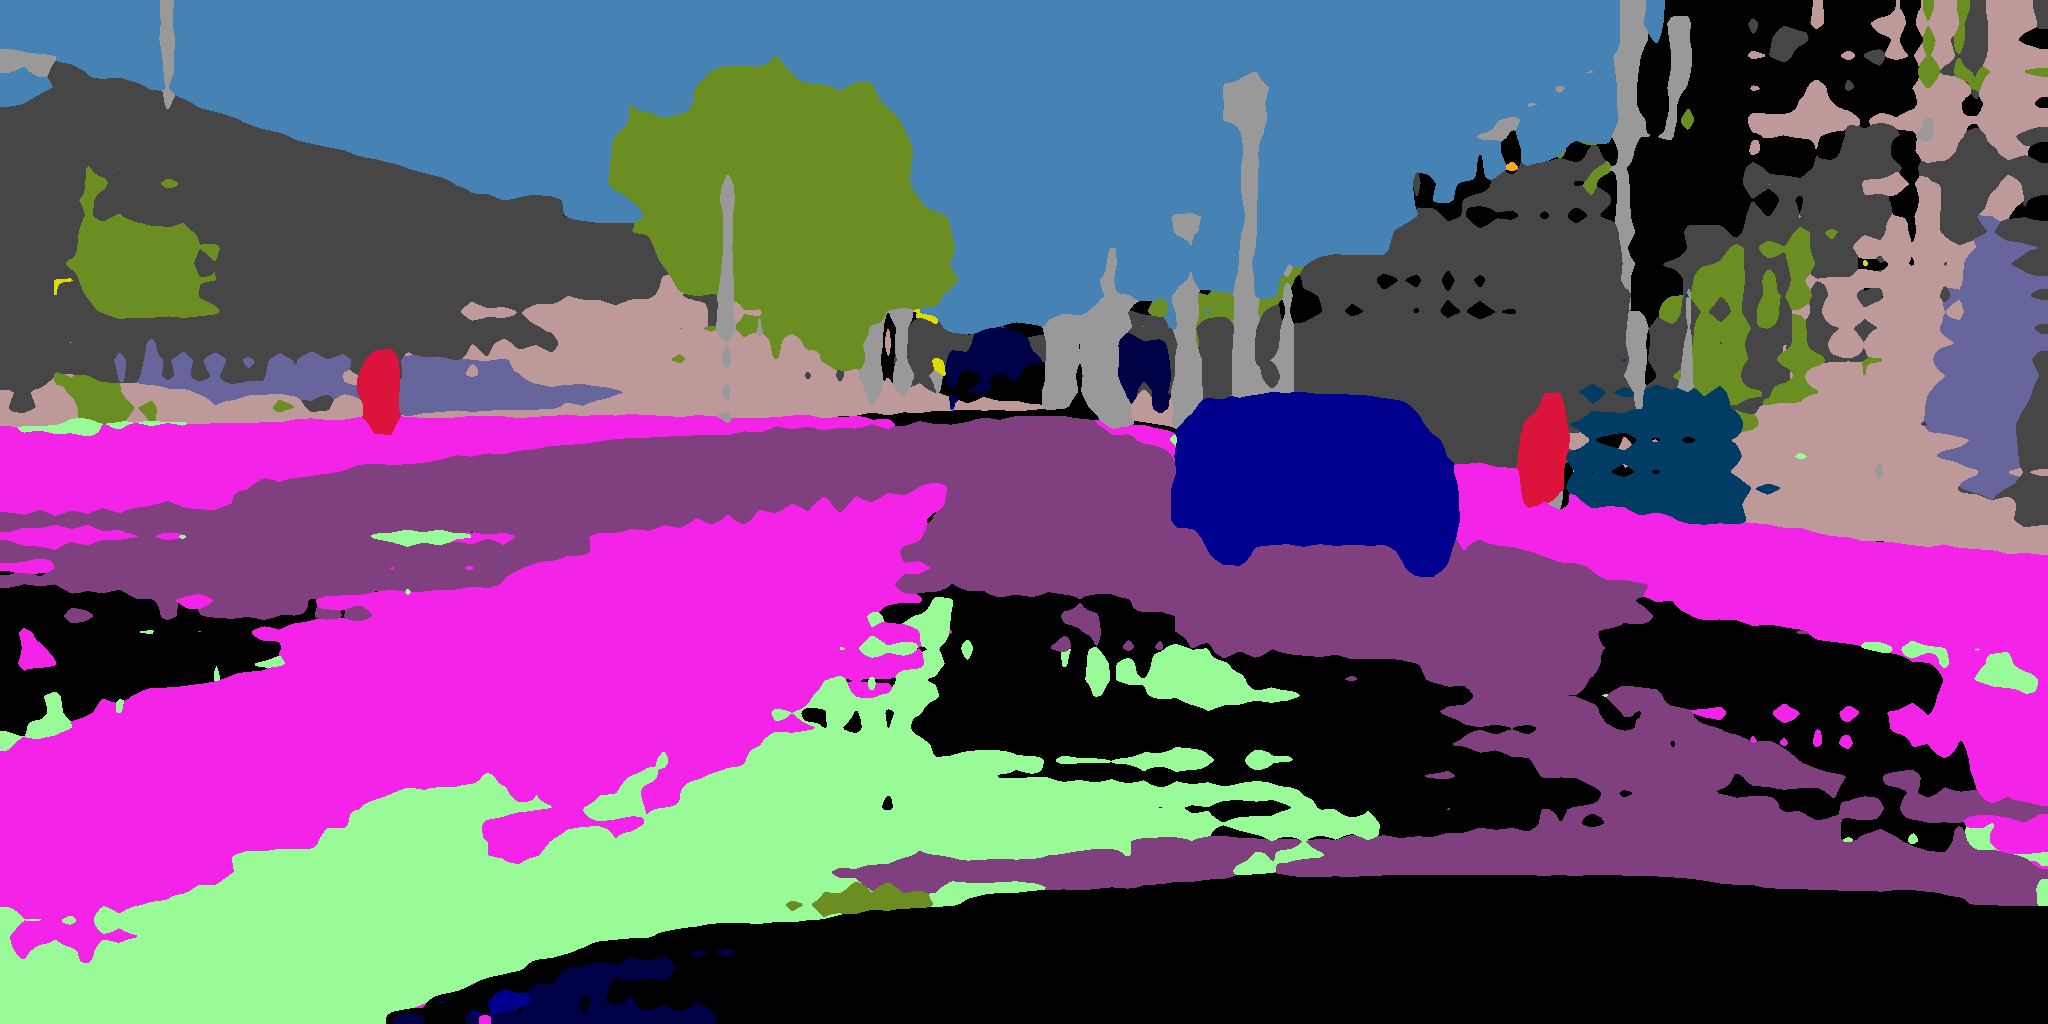
\includegraphics[width=\textwidth]{../images/evaluation/GTA_pred_labels.png}
			\end{minipage}\\
			\rotatebox[origin=c]{90}{\tiny CycleGAN} &
			\begin{minipage}[c]{\textwidth}
				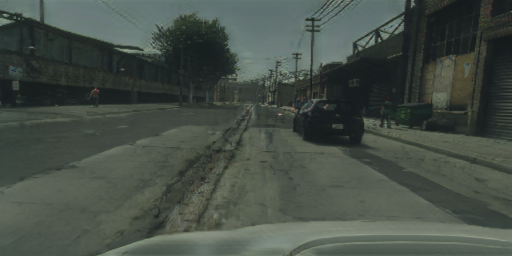
\includegraphics[width=\textwidth]{../images/evaluation/CycleGAN_translated.png}
			\end{minipage} &
			\begin{minipage}[c]{\textwidth}
				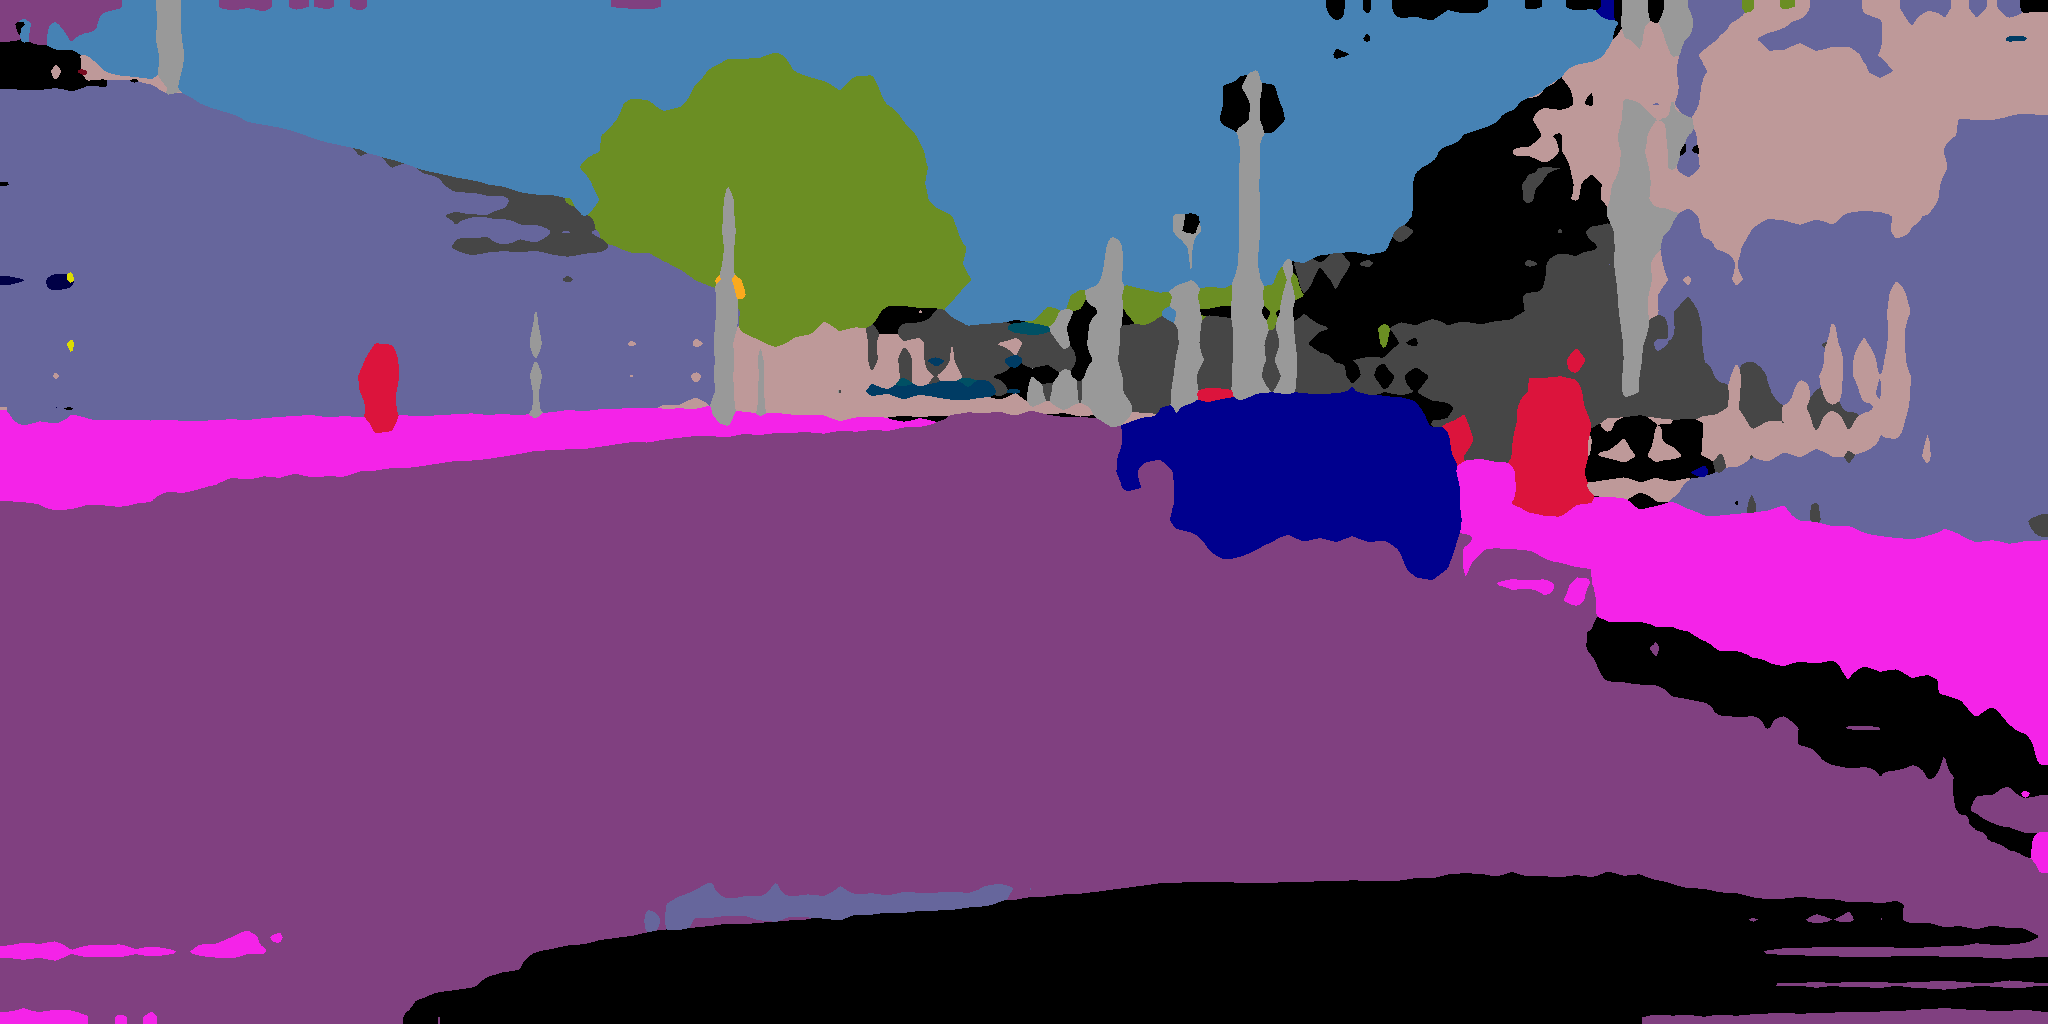
\includegraphics[width=\textwidth]{../images/evaluation/CycleGAN_pred_labels.png}
			\end{minipage}\\
			\rotatebox[origin=c]{90}{\tiny CyCADA} &
			\begin{minipage}[c]{\textwidth} 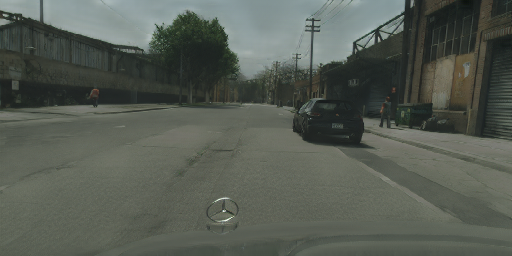
\includegraphics[width=\textwidth]{../images/evaluation/CyCADA_translated.png} 
			\end{minipage}& 
			\begin{minipage}[c]{\textwidth}
				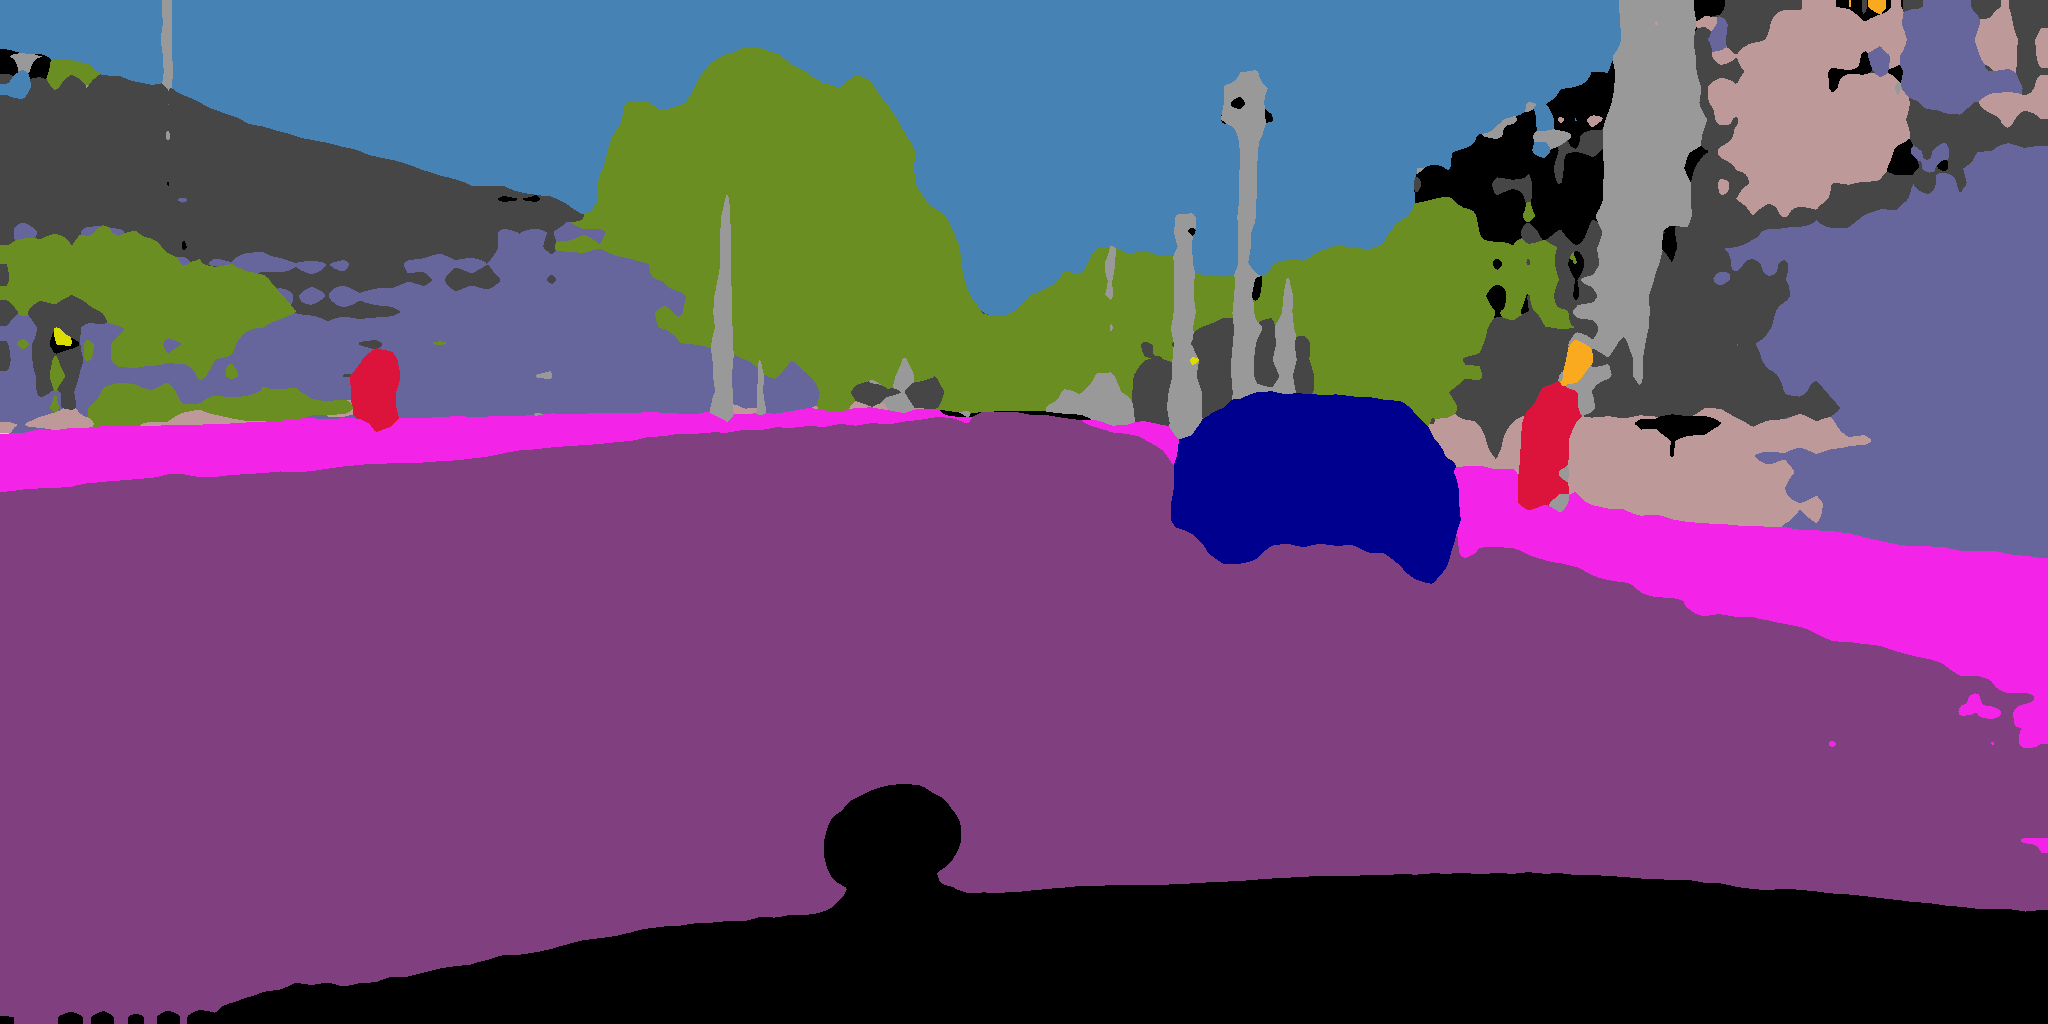
\includegraphics[width=\textwidth]{../images/evaluation/CyCADA_pred_labels.png}
			\end{minipage}\\
			\rotatebox[origin=c]{90}{\tiny SG-GAN} &
			\begin{minipage}[c]{\textwidth} 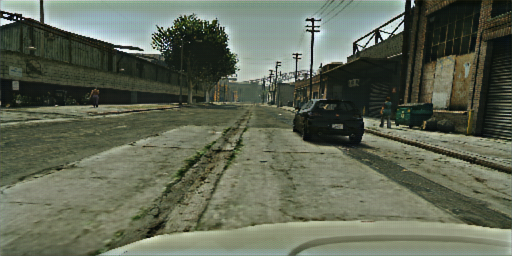
\includegraphics[width=\textwidth]{../images/evaluation/SG-GAN_translated.png}
			\end{minipage} & 
			\begin{minipage}[c]{\textwidth}
				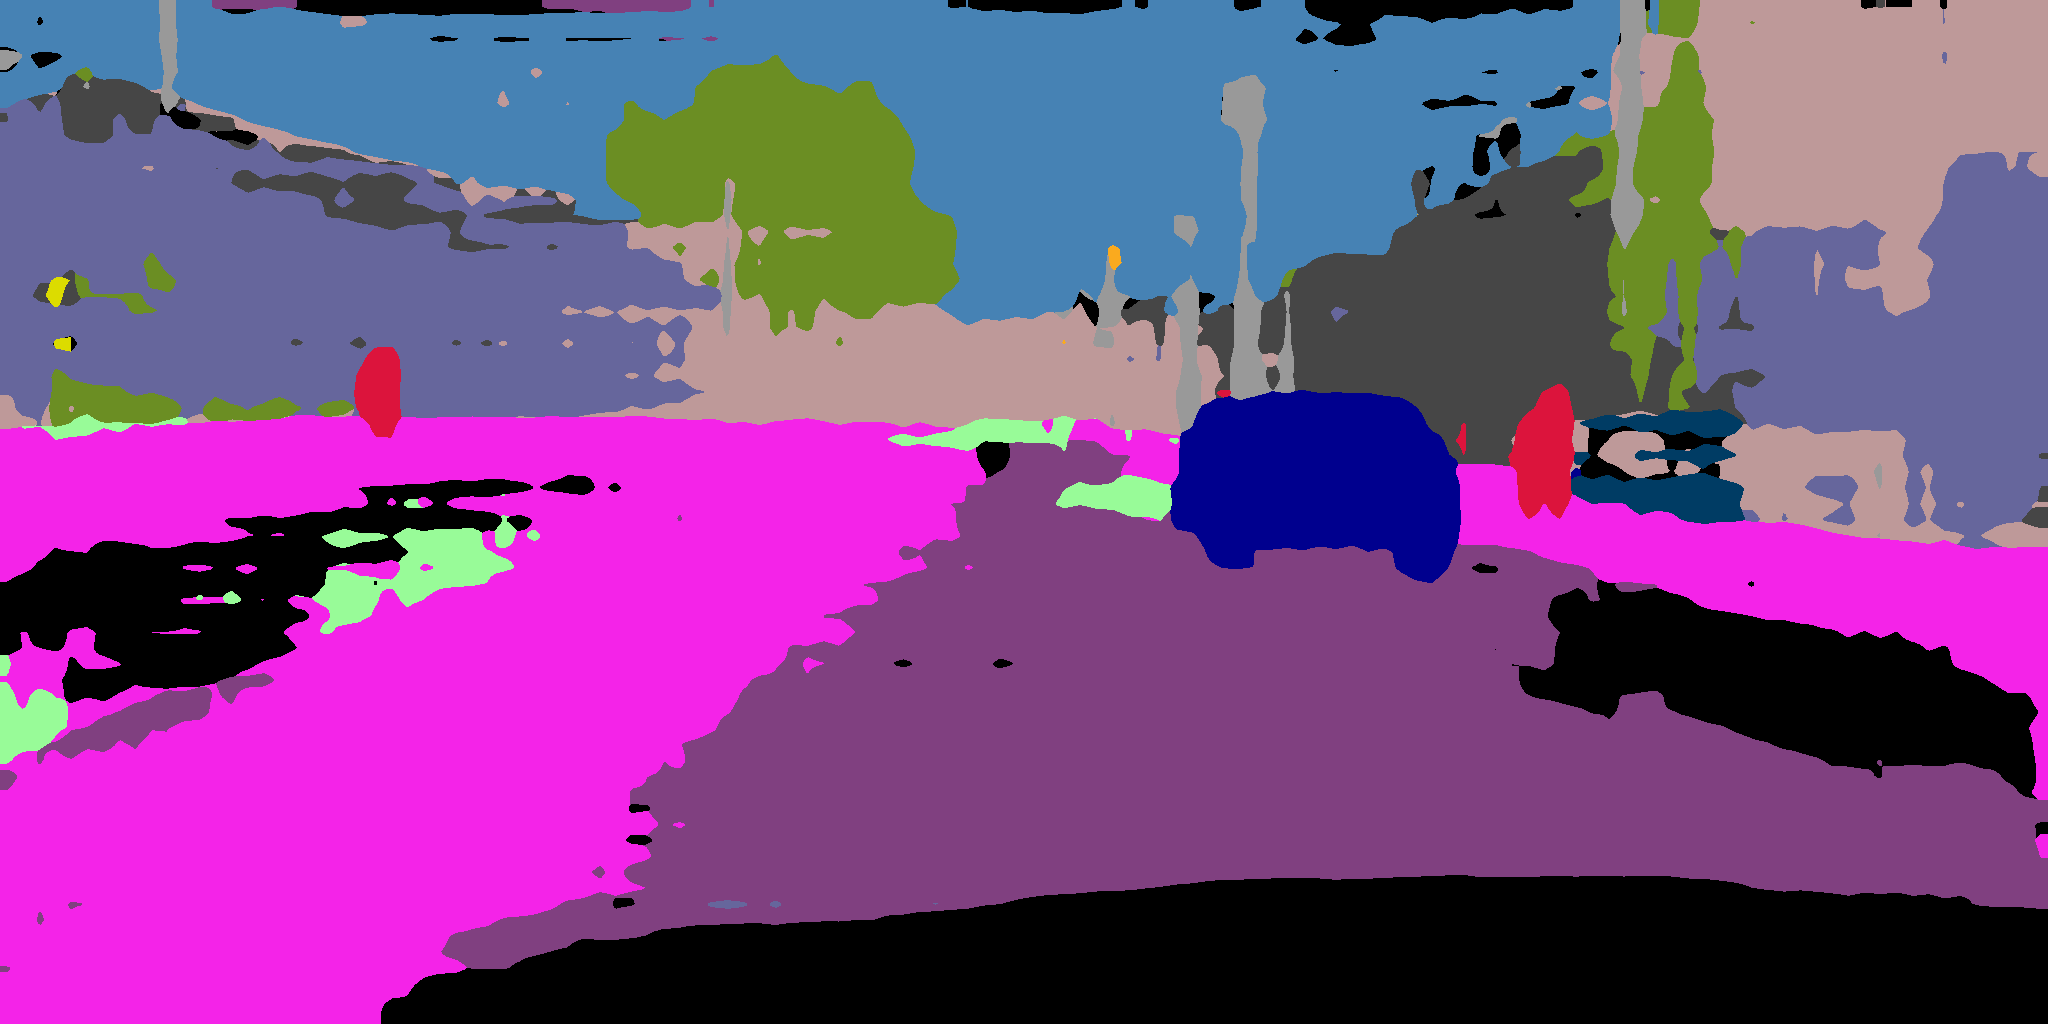
\includegraphics[width=\textwidth]{../images/evaluation/SG-GAN_pred_labels.png}
			\end{minipage} \\
			%\multicolumn{2}{c}{} \\
			\multicolumn{1}{c}{} & \tiny (translated) Image & \tiny (predicted) Label map
		\end{tabular}}
	%\caption{ground-truth image and corresponding ground-truth label map from the GTA5 dataset (top) and the images translated by the different techniques (left side) with their corresponding predicted label maps (right side)}
	\end{table}
	\column{.5\textwidth}
	\begin{table}
		\begin{tabular}{c}
			GTA5 (ground-truth) \\
			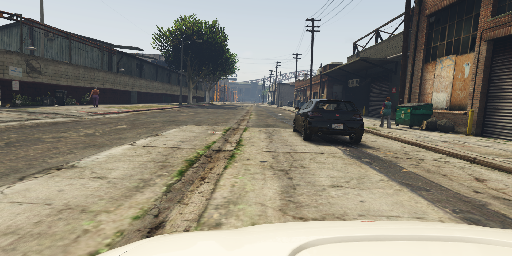
\includegraphics[width=0.9\textwidth]{../images/evaluation/GTA_gt_image.png}\\
			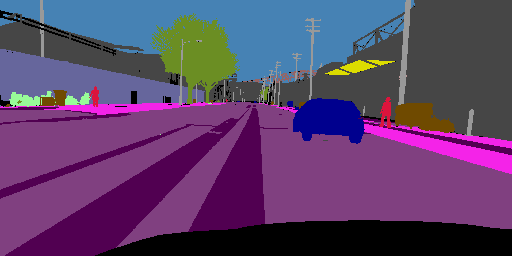
\includegraphics[width=0.9\textwidth]{../images/evaluation/GTA_gt_label.png}
		\end{tabular}
	\end{table}
\end{columns}
\end{frame}

\begin{frame}
\frametitle{Qualitative}
\begin{columns}[c]
	\column{.5\textwidth}
	\begin{table}
		\resizebox{1.15\textwidth}{!}{%
			\begin{tabular}{cc||c}
				\rotatebox[origin=c]{90}{\tiny GTA5} &
				\multicolumn{1}{c||}{} &
				\begin{minipage}[c]{\textwidth}
					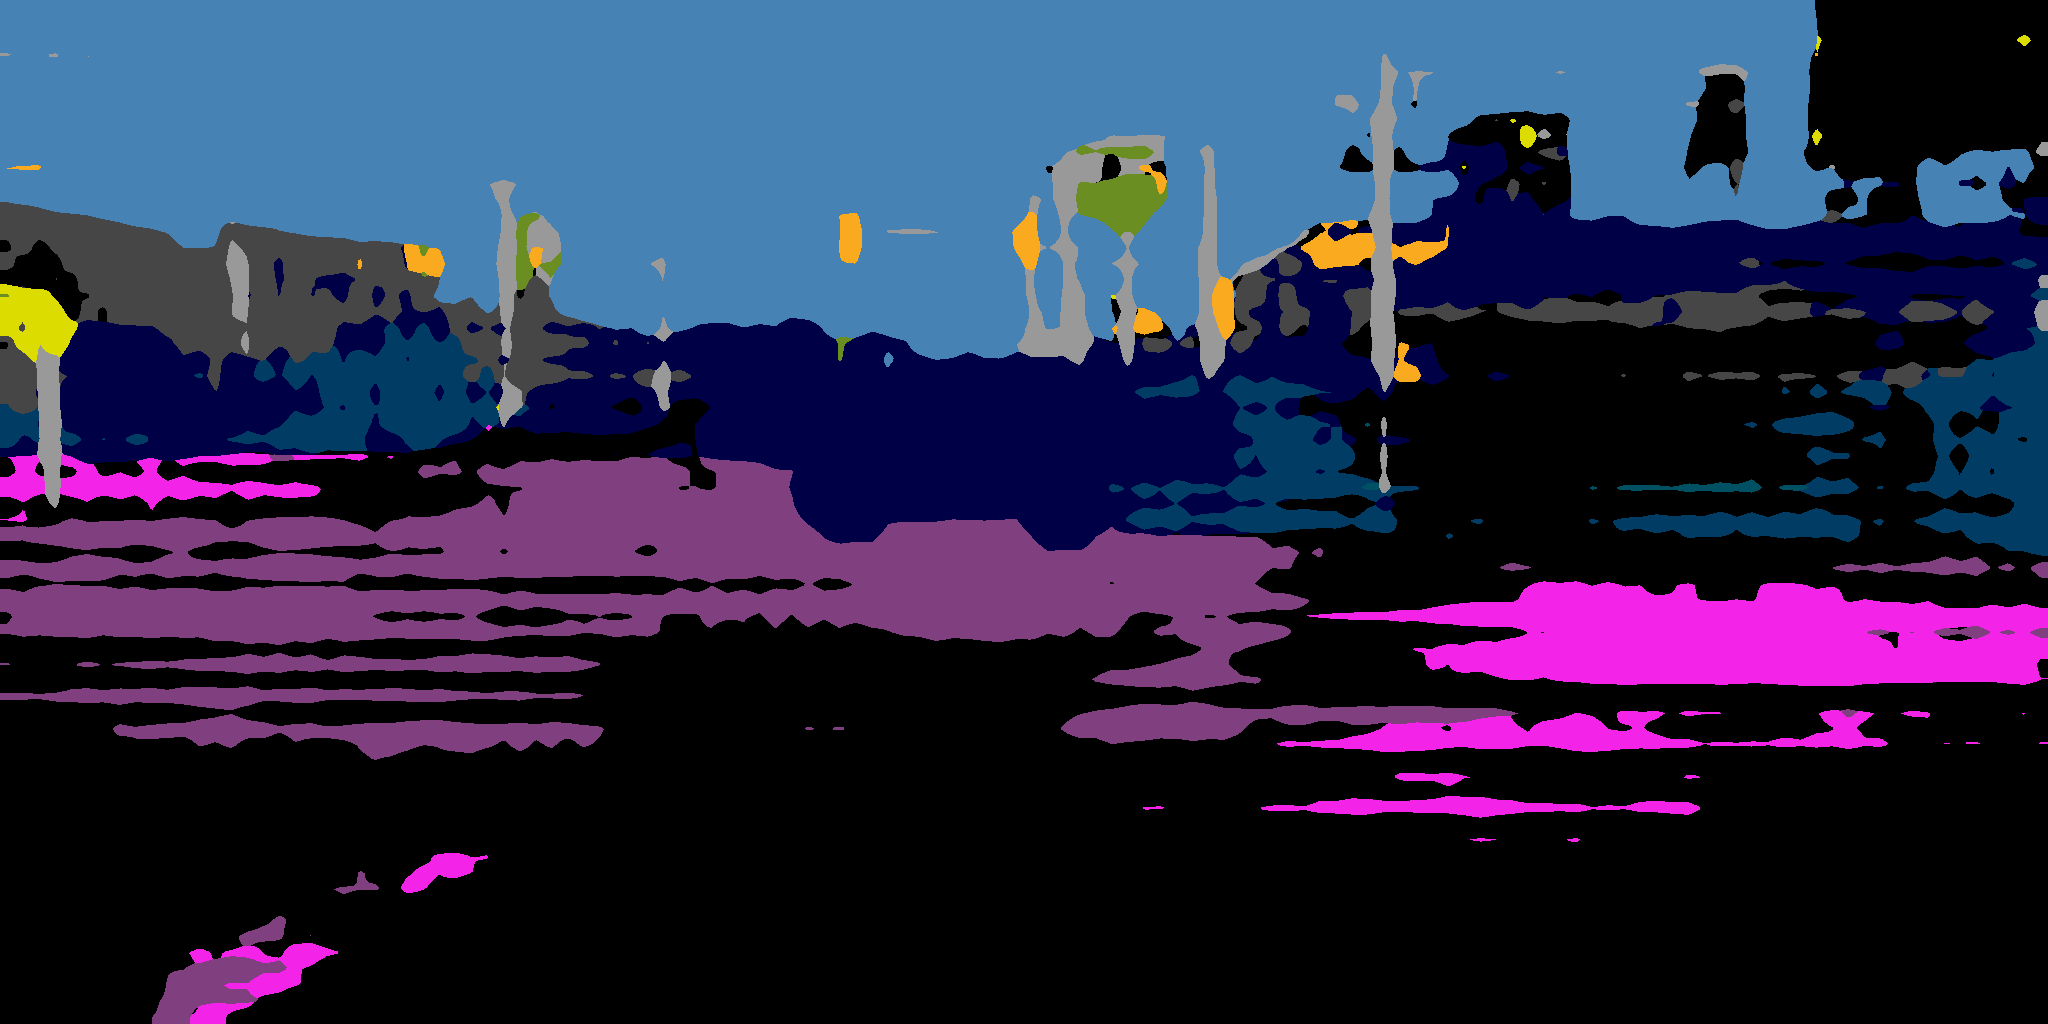
\includegraphics[width=\textwidth]{../images/evaluation/GTA_pred_labels_train.png}
				\end{minipage}\\
				\rotatebox[origin=c]{90}{\tiny CycleGAN} &
				\begin{minipage}[c]{\textwidth}
					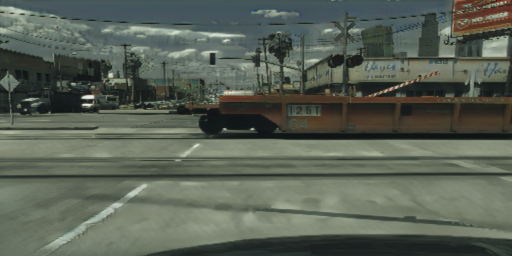
\includegraphics[width=\textwidth]{../images/evaluation/CycleGAN_translated_train.png}
				\end{minipage} &
				\begin{minipage}[c]{\textwidth}
					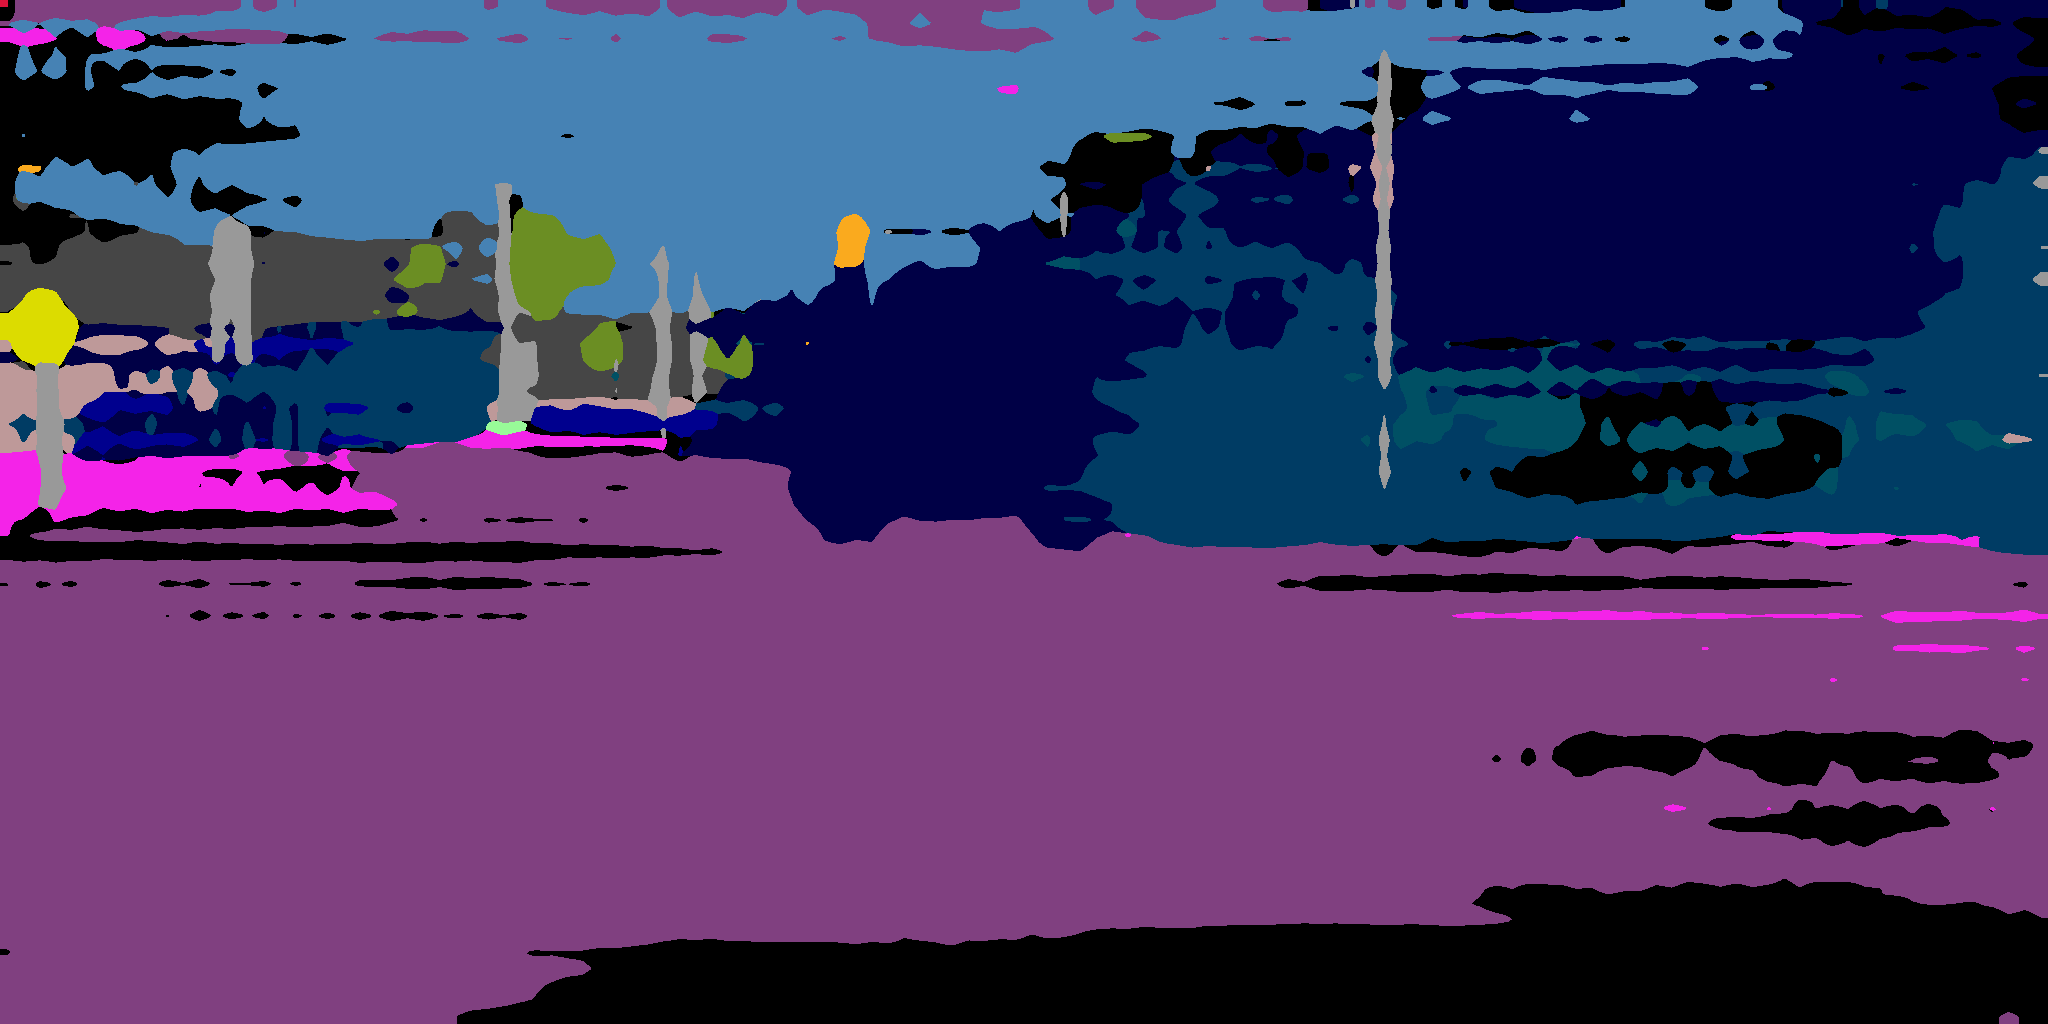
\includegraphics[width=\textwidth]{../images/evaluation/CycleGAN_pred_labels_train.png}
				\end{minipage}\\
				\rotatebox[origin=c]{90}{\tiny CyCADA} &
				\begin{minipage}[c]{\textwidth} 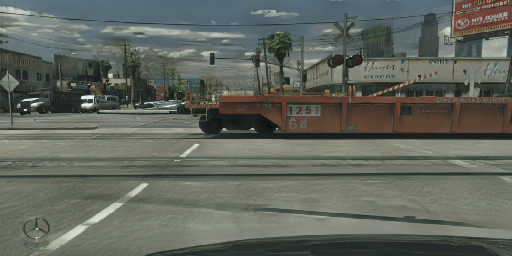
\includegraphics[width=\textwidth]{../images/evaluation/CyCADA_translated_train.png}
				\end{minipage}& 
				\begin{minipage}[c]{\textwidth}
					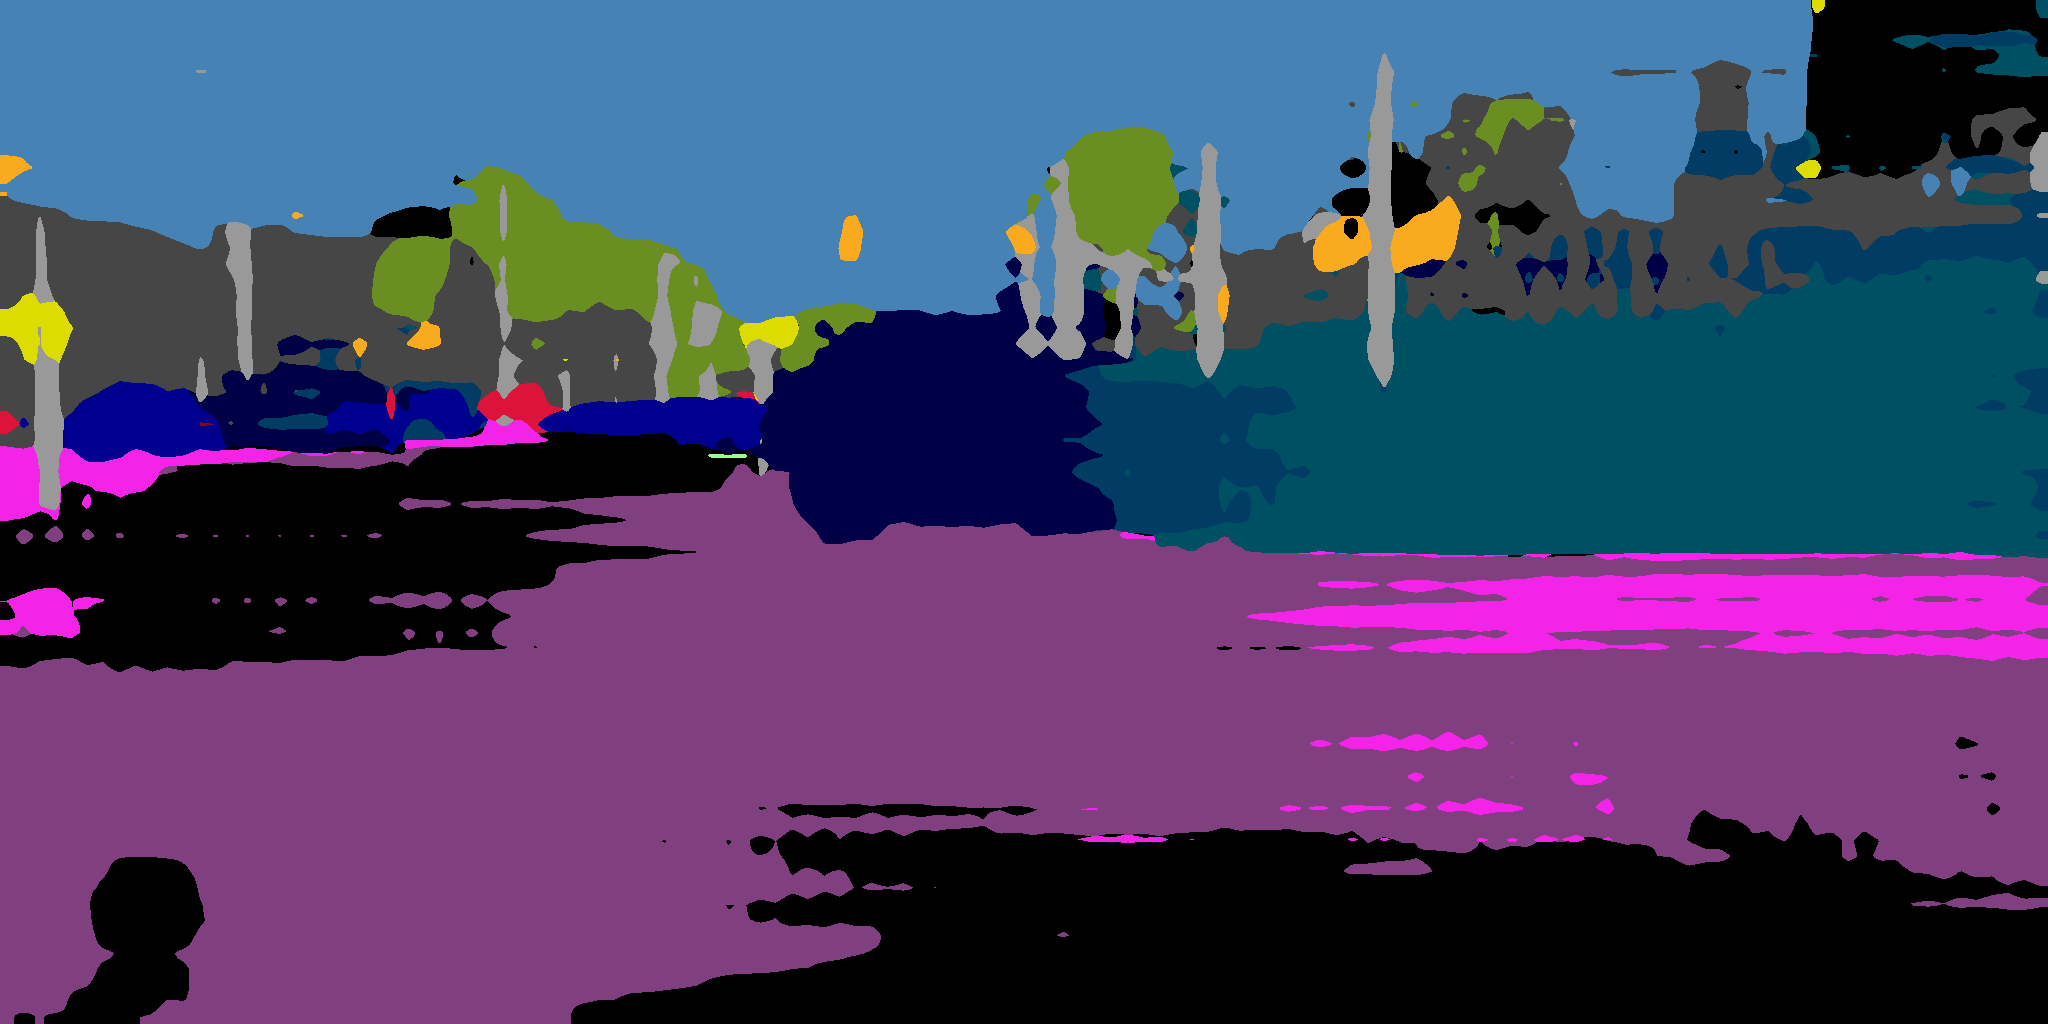
\includegraphics[width=\textwidth]{../images/evaluation/CyCADA_pred_labels_train.png}
				\end{minipage}\\
				\rotatebox[origin=c]{90}{\tiny SG-GAN} &
				\begin{minipage}[c]{\textwidth} 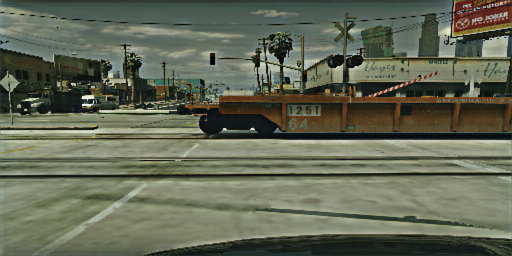
\includegraphics[width=\textwidth]{../images/evaluation/SG-GAN_translated_train.png}
				\end{minipage} & 
				\begin{minipage}[c]{\textwidth}
					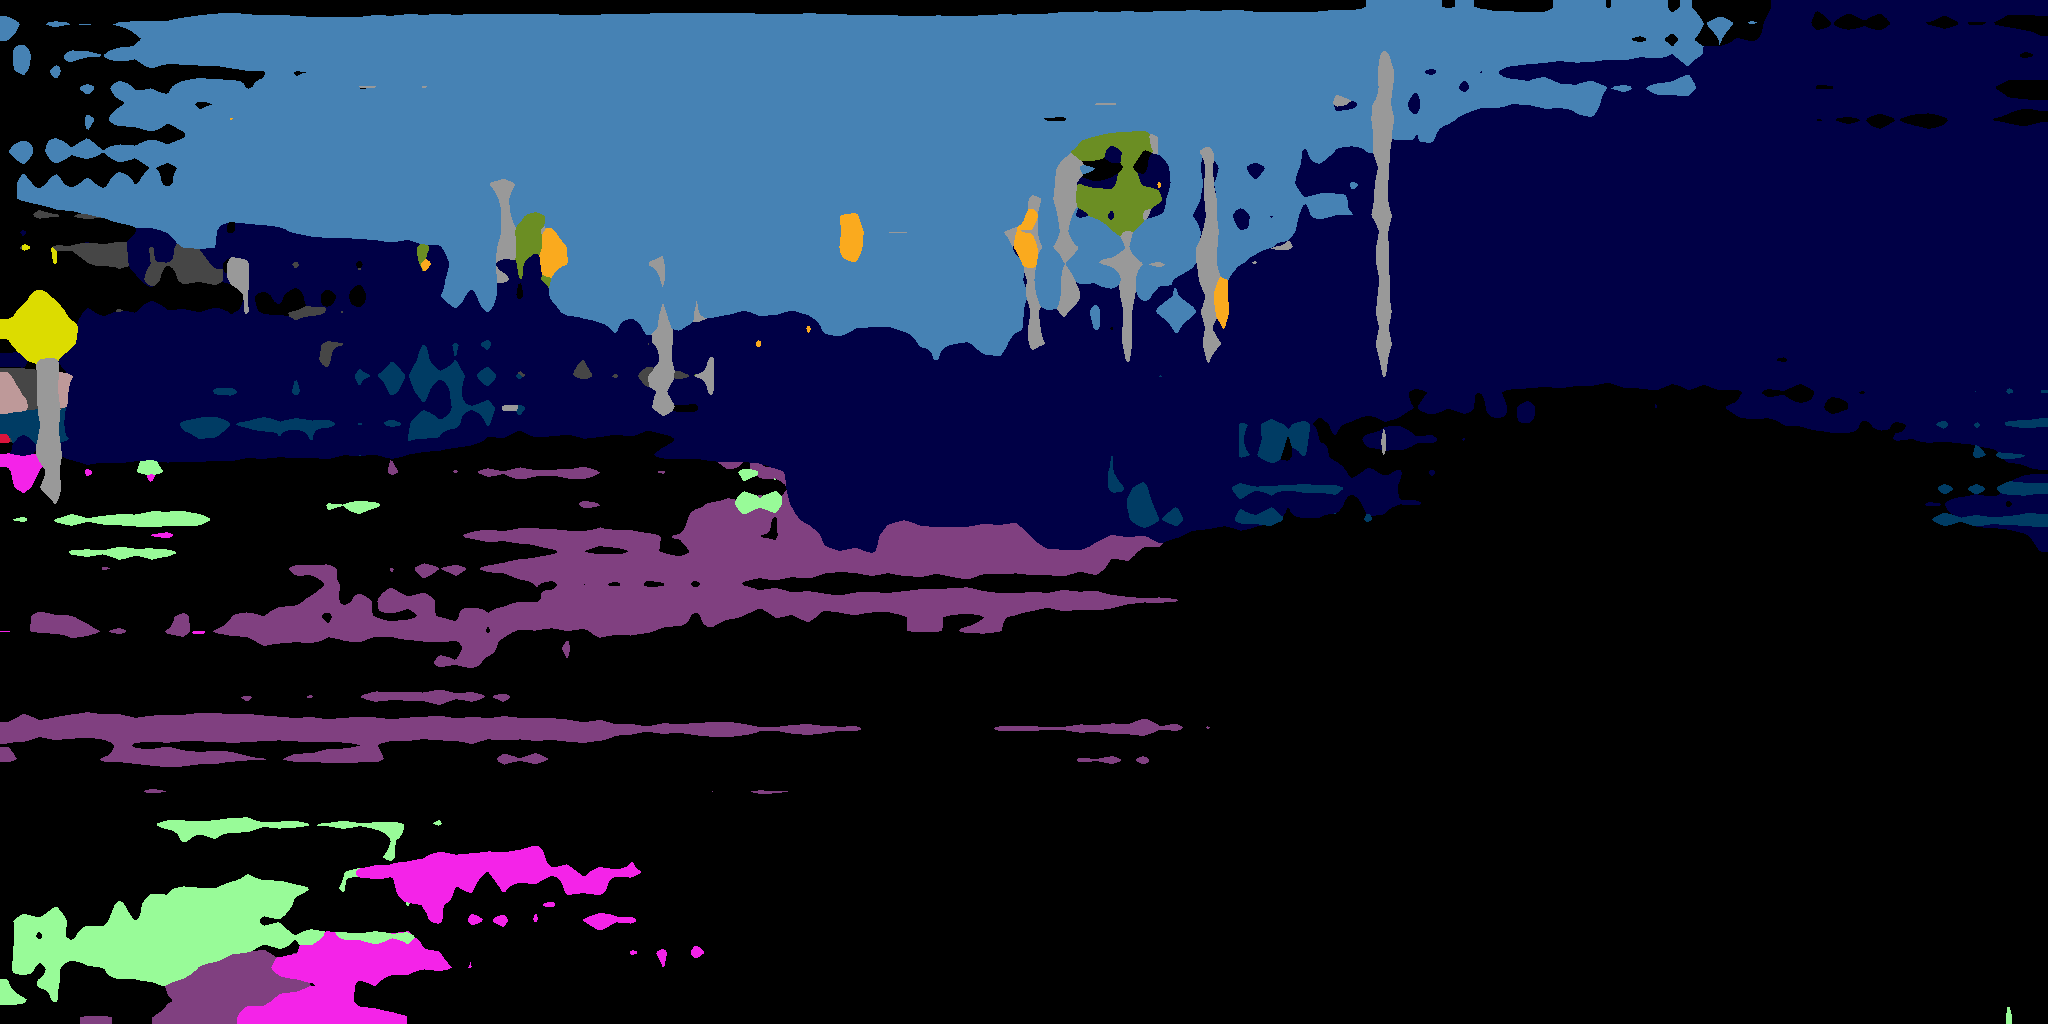
\includegraphics[width=\textwidth]{../images/evaluation/SG-GAN_pred_labels_train.png}
				\end{minipage} \\
				%\multicolumn{2}{c}{} \\
				\multicolumn{1}{c}{} & \tiny (translated) Image & \tiny (predicted) Label map
		\end{tabular}}
		%\caption{ground-truth image and corresponding ground-truth label map from the GTA5 dataset (top) and the images translated by the different techniques (left side) with their corresponding predicted label maps (right side)}
	\end{table}
	\column{.5\textwidth}
	\begin{table}
		\begin{tabular}{c}
			GTA5 (ground-truth) \\
			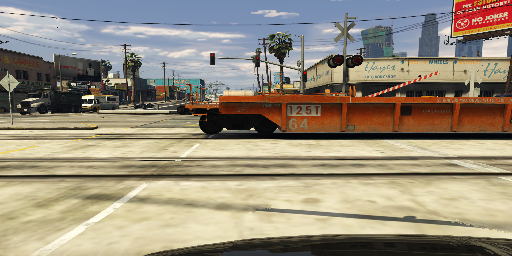
\includegraphics[width=0.9\textwidth]{../images/evaluation/GTA_gt_image_train.png}\\
			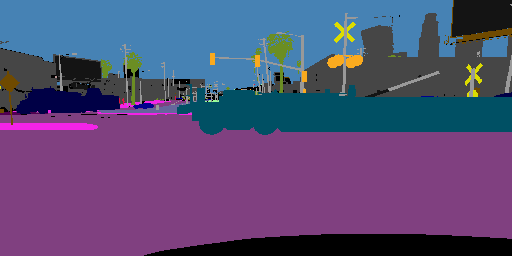
\includegraphics[width=0.9\textwidth]{../images/evaluation/GTA_gt_label_train.png}
		\end{tabular}
	\end{table}
\end{columns}
\end{frame}

%------------------------------------------------
\section{Discussion}
%------------------------------------------------

\subsection{Training}

\begin{frame}
\frametitle{Pre-trained models}
\begin{itemize}
	\item the models used might not represent the ones described in papers
	\item therefore adaptation not as accurate
\end{itemize}
\end{frame}

\begin{frame}
\frametitle{DeepLabV3 model}
\begin{itemize}
	\item trained less precise than in its paper
	\item overall performance scores are lower than expected
	\item relation between model performance should remain the same though
\end{itemize}
\end{frame}

\begin{frame}
\frametitle{sampleset of images / techniques with different strengths}
\begin{itemize}
	\item sampleset of images might be too small
	\item techniques have different strength, e.g. SG-GAN: traffic signs class, CyCADA: train class
	\item this might alter the average scores
\end{itemize}
\end{frame}

%------------------------------------------------
\section{Conclusion}
%------------------------------------------------

\begin{frame}
\frametitle{to conclude}
\begin{itemize}
	\item compared three techniques on Synthetic-to-Real Domain Adaptation
	\item expected all models to increase performance compared to pure GTA5
	\item CyCADA only one to improve average scores
	\item SG-GAN improved performance on some classes
	\item CycleGAN did not perform best for any class or category
	\item getting the repo code to run was a challenge
\end{itemize}
\end{frame}

\begin{frame}
\frametitle{Outlook and Future Work}
\begin{itemize}
	\item train models from scratch: better comparison as framework is known exactly
	\item compare more models: newly developed ones and other existing ones (there might exist better ones)
	\item other comparison benchmarks: e.g. perceptual loss (compare features in images)
	\item sampleset size of test images: lower chance of favorable corner cases that increase average score of a specific technique
\end{itemize}
\end{frame}



%\begin{frame}
%\frametitle{The SYNTHIA dataset: A large collection of synthetic images for semantic segmentation of urban scenes}
%\cite{synthia}
%\begin{columns}[c]
%\column{.5\textwidth}
%%\begin{figure}
%%	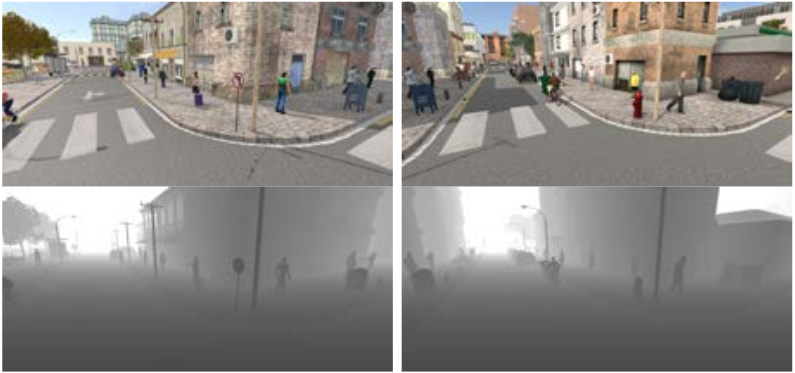
\includegraphics[width=\linewidth]{../images/SYNTHIA_depth_half.png}
%%	\caption{RGB images (top), corresponding depth-maps (bottom)}
%%\end{figure}
%\column{.5\textwidth}
%%\begin{figure}
%%	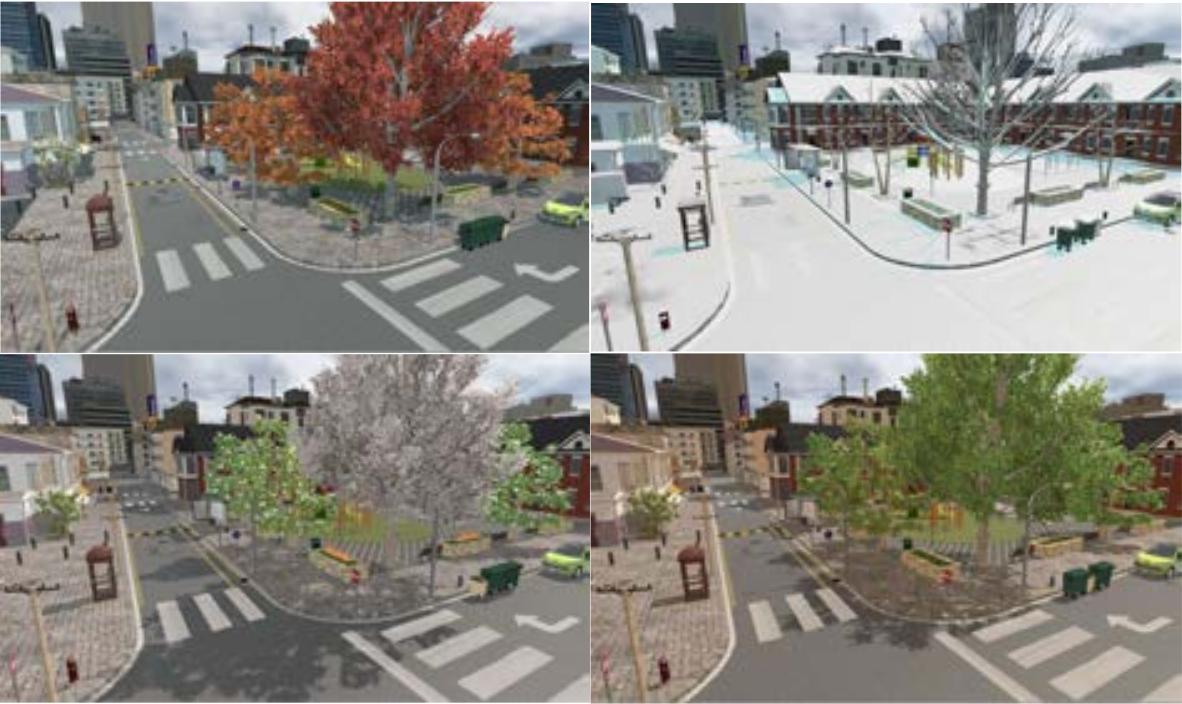
\includegraphics[width=\linewidth]{../images/SYNTHIA_seasons.png}
%%	\caption{from top left to bottom right: fall, winter, spring, summer}
%%\end{figure}
%\end{columns}
%\end{frame}
\begin{frame}
	\begin{center}
		\textbf{Thank you}
	\end{center}
\end{frame}

%------------------------------------------------

\begin{frame}
\titlepage
\end{frame}

%----------------------------------------------------------------------------------------

\section*{References}

%\begin{frame}
%\frametitle{References}
%\footnotesize{
%\begin{thebibliography}{99} 
%	\bibitem[Butler et. al]{sintel} Butler et al.
%	\newblock A naturalistic open source movie for optical flow evaluation
%	\newblock \emph{European Conf. on Computer Vision (ECCV)} Part IV, LNCS 7577, 611 -- 625. Springer-Verlag, October 2012
%\end{thebibliography}
%
%\begin{thebibliography}{99} 
%	\bibitem[Ley et al.]{syb3r} Ley et al.
%	\newblock
%	\newblock \emph{SyB3R: A Realistic Synthetic Benchmark for 3D Reconstruction from Images}, pages 236 -- 251. Springer International Publishing, 2016
%\end{thebibliography}
%
%\begin{thebibliography}{99} 
%	\bibitem[Ros et. al]{synthia} Ros et al.
%	\newblock The SYNTHIA Dataset: A large collection of synthetic images for semantic segmentation of urban scenes
%	\newblock 2016
%\end{thebibliography}
%
%\begin{thebibliography}{99} 
%	\bibitem[Richter et. al]{p4d} Richter et al.
%	\newblock Playing for data: Ground truth from computer games
%	\newblock In Bastian Leibe et al., editors \emph{European Conf. on Computer Vision (ECCV)}, LNCS 9906, 102 -- 118. Springer International Publishing, 2016
%\end{thebibliography}
%}
%\end{frame}
%
%
%
%\begin{frame}
%\frametitle{References}
%\footnotesize{
%	\begin{thebibliography}{99} 
%		\bibitem[Huang et. al]{deepmvs} Huang et al.
%		\newblock DeepMVS: Learning Multi-view Stereopsis
%		\newblock \emph{CoRR}, abs/1804.00650, 2018
%	\end{thebibliography}
%	\begin{thebibliography}{99} 
%		\bibitem[Isola et. al]{i2i} Isola et al.
%		\newblock Image-to-image translation with conditional adversarial networks
%		\newblock \emph{CoRR}, abs/1611.07004, 2016
%	\end{thebibliography}
%
%	\begin{thebibliography}{99} 
%		\bibitem[Zhu et. al]{ui2i} Zhu et al.
%		\newblock Unpaired image-to-image translation using cycle-consistent adversarial networks
%		\newblock \emph{CoRR}, abs/1703.10593, 2017
%	\end{thebibliography}
%}
%\end{frame}

\end{document} 